\mysection{Úvod}

V našom ročníkovom projekte sme sa rozhodli zaoberať vi\-zu\-a\-li\-zá\-ciou distribuovaných algortimov
pomocou Java aplikácie, ktorá umožňuje jednoduché a rýchle pochopenie témy, bez
študovania dlhých odborných textov.

\begin{figure}
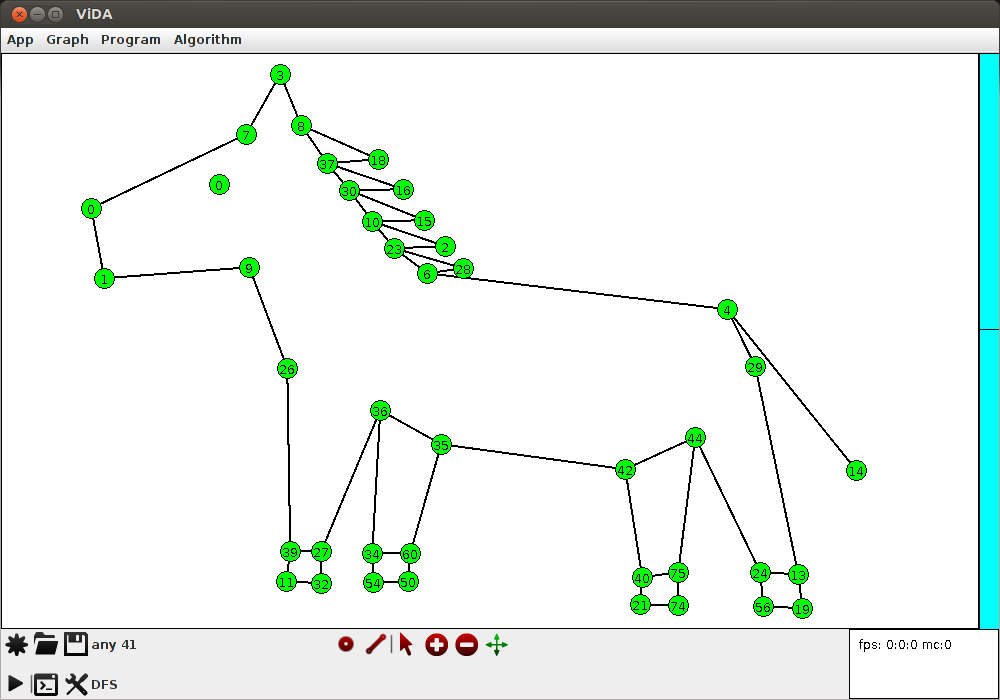
\includegraphics[width=\columnwidth]{konik}
%\vspace{-1cm}
%\caption{Vzhľad aplikácie po spustení a naklikaní grafu koníka}
\end{figure}

\mysection{Distribuované algoritmy}

Vlastnosti modelu:
\begin{itemize}
    \item niekoľko počítačov zapojených do siete obojsmernými linkami
    \item majú jednoznačné id, komunikujú len správami
    \item správy sa nestrácajú, nemenia poradie, ale môže im to trvať ľubovoľne dlho -- asynchrónna
    komunikácia
\end{itemize}

Ciele:
\begin{itemize}
    \item poslať čo najmenej správ
    \item minimalizovať dobu behu algoritmu
\end{itemize}

\begin{figure}
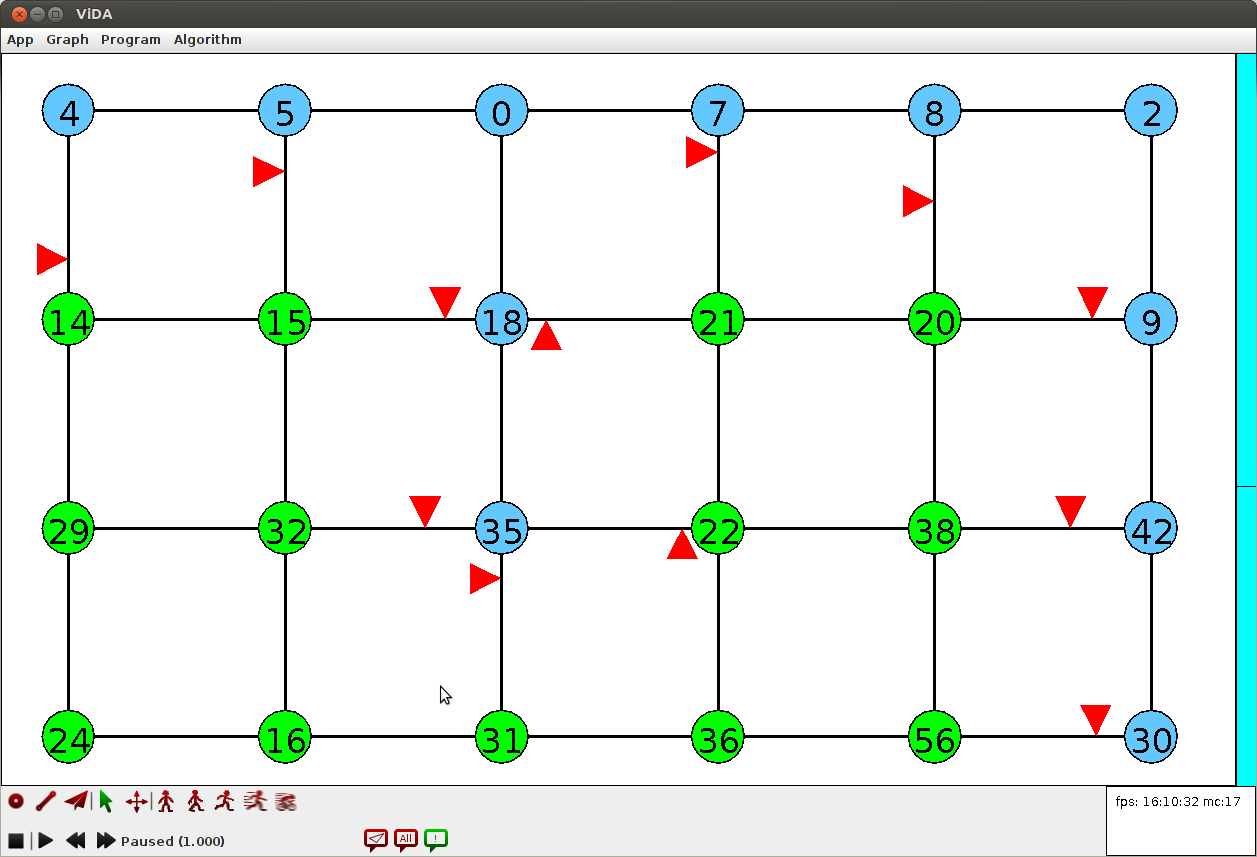
\includegraphics[width=\columnwidth]{asyn}
\vspace{-1cm}
\caption{Asynchrónna komunikácia -- klebeta začala vľavo hore (vrchol~4) a dostala sa na druhý
koniec mriežky (vrchol~30) skôr, než do spodného suseda (vrchol~14). Aj toto naša vizualizácia
dokáže spraviť. }
\end{figure}
%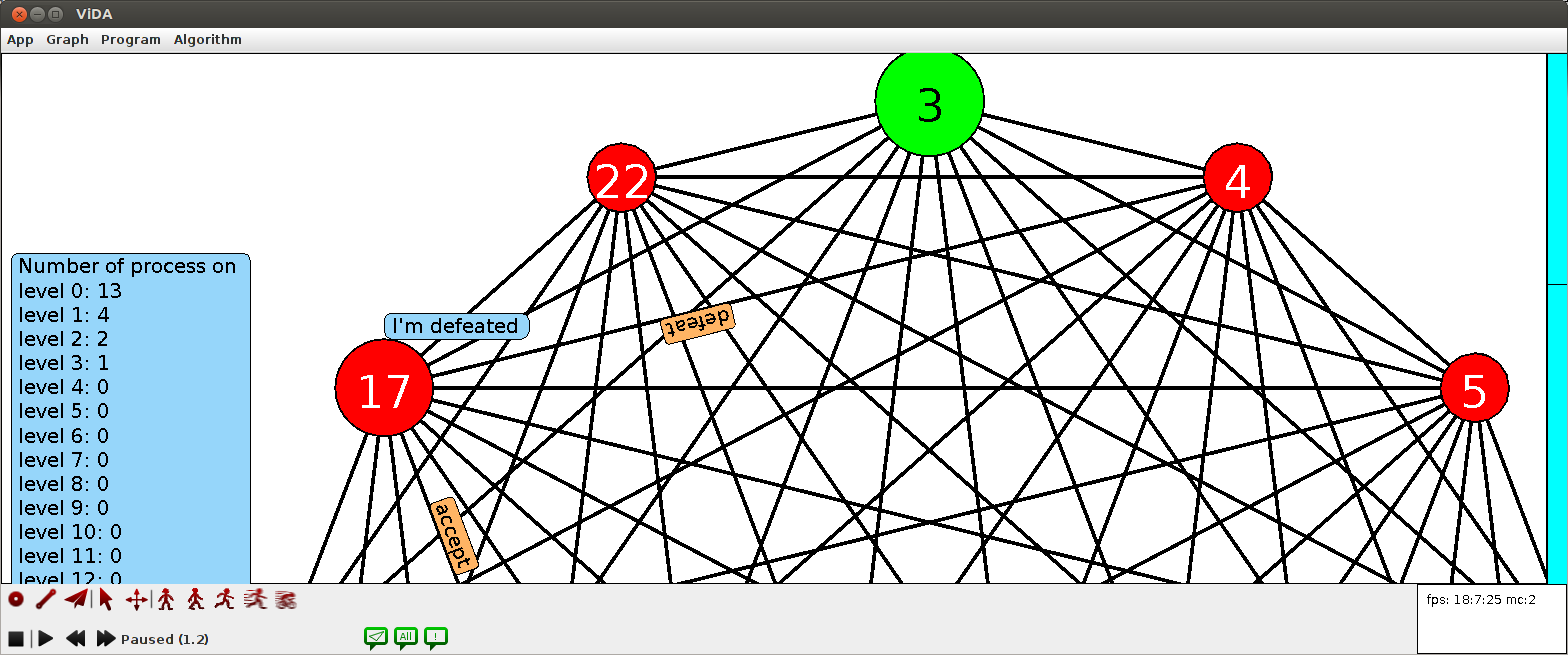
\includegraphics[width=\columnwidth]{le}

\mysection{Hlavné ciele}
\begin{itemize}
    \item vizualizácie ušité na mieru konkrétnym distribuovaným algoritmom
    \item interaktivita s používateľom
    \item prehľadnosť a jednoduchosť používania aplikácie
    \item schopnosť vizualizovať vlastné algoritmy
\end{itemize}
\vspace{-0.5cm}
